
{\color{red} Still to be added:
\begin{itemize}
\item {Alignment Strategy description?}
\item Survey description and lessons learned?
\item Updated figures
\item Track based results (if there)
\item Conclusions 
\end{itemize}
}

The main handle on the internal alignment of the silicon sensors is the so-called track residual. It is defined as the difference of the measured hit position and the predicted track 
position at that sensor. As described in Sec.~\ref{sec:svt_clustering} the individual hits on the 
strip sensors are combined into a 3D space point. Figure~\ref{fig:res_top_nonbend} and~\ref{fig:res_top_bend} shows the 3D space point track residuals in the non-bend and bend plane, respectively, for tracks in the top half of the tracker.
\begin{figure*}[t]
%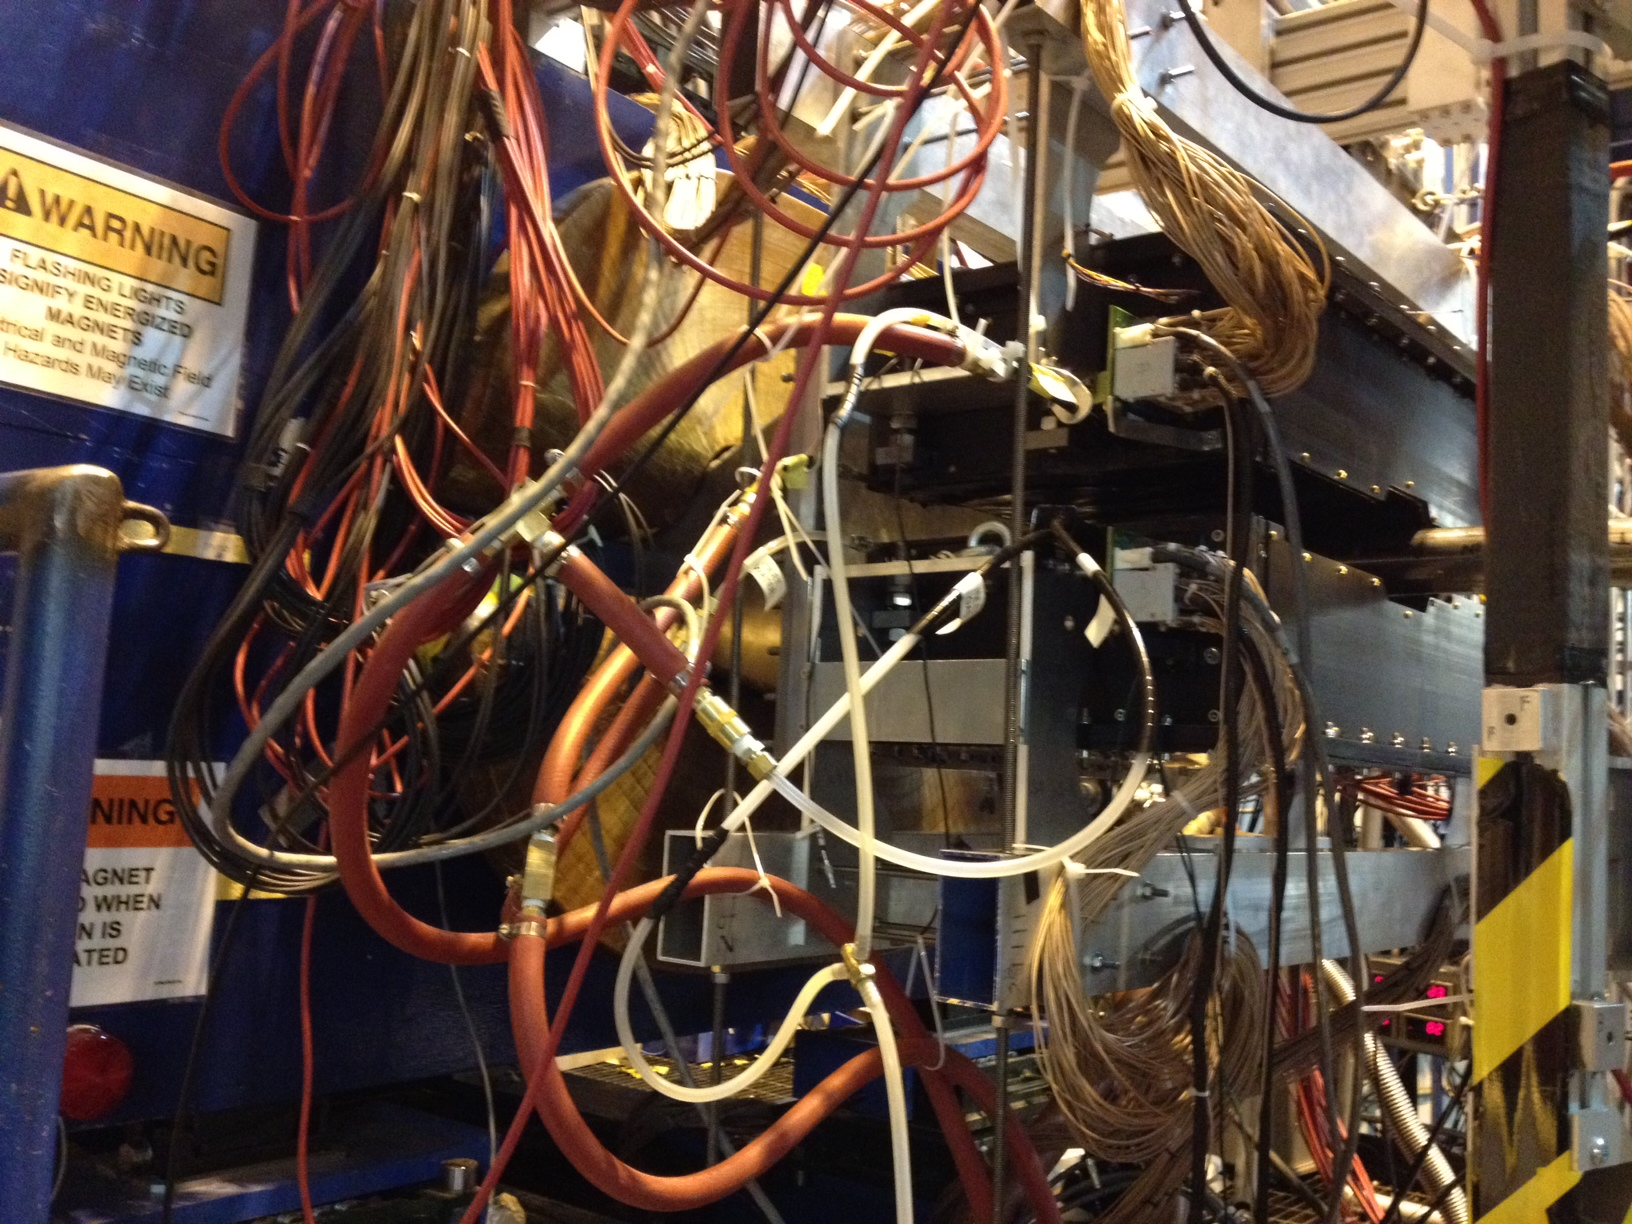
\includegraphics[ scale=0.25]{test2012/ecal_mounted.JPG}
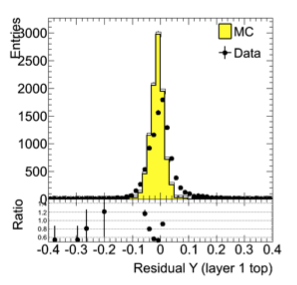
\includegraphics[ scale=0.5]{test2012/alignment/pictures/res_top/res_top-1.png}
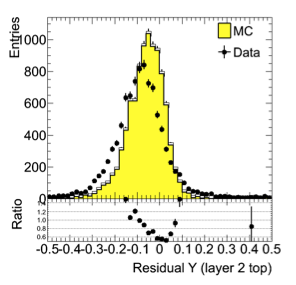
\includegraphics[ scale=0.5]{test2012/alignment/pictures/res_top/res_top-2.png}
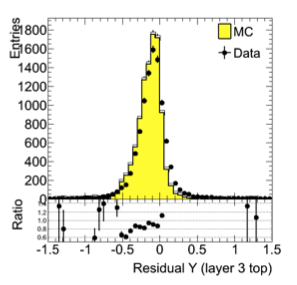
\includegraphics[ scale=0.5]{test2012/alignment/pictures/res_top/res_top-3.png}
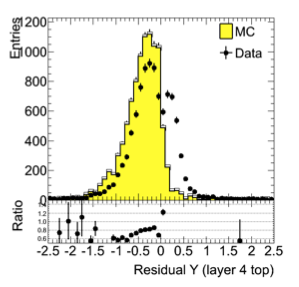
\includegraphics[ scale=0.5]{test2012/alignment/pictures/res_top/res_top-4.png}
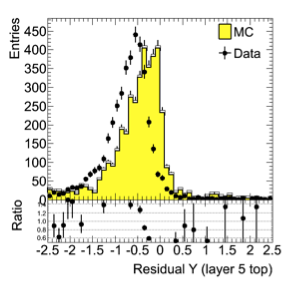
\includegraphics[ scale=0.5]{test2012/alignment/pictures/res_top/res_top-5.png}
\caption{\small{Residuals in the bend plane for tracks reconstructed in the 
top half of the tracker. }}\label{fig:res_top_bend}
\end{figure*}
\begin{figure*}[t]
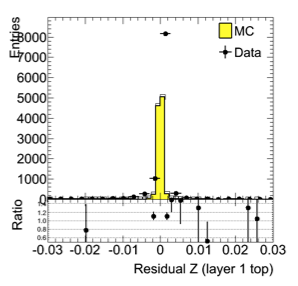
\includegraphics[ scale=0.5]{test2012/alignment/pictures/res_top/res_top-6.png}
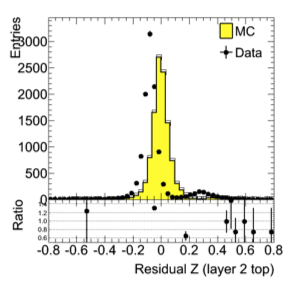
\includegraphics[ scale=0.5]{test2012/alignment/pictures/res_top/res_top-7.png}
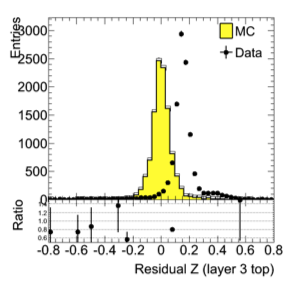
\includegraphics[ scale=0.5]{test2012/alignment/pictures/res_top/res_top-8.png}
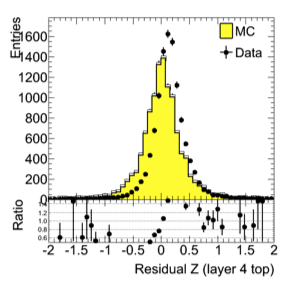
\includegraphics[ scale=0.5]{test2012/alignment/pictures/res_top/res_top-9.png}
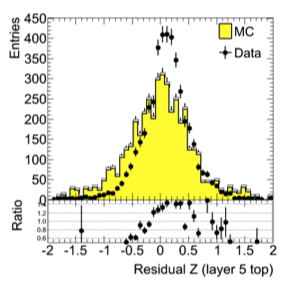
\includegraphics[ scale=0.5]{test2012/alignment/pictures/res_top/res_top-10.png}
\caption{\small{Residuals in the bend non-plane for tracks reconstructed in the 
top half of the tracker.  }}\label{fig:res_top_nonbend}
\end{figure*}
As can be seen from the simulation the ideal aligned tracker would have mean residuals 
of zero. Figure~\ref{fig:res_top_summary} shows the mean of the residuals for 
each layer of the tracker. 
\begin{figure*}[t]
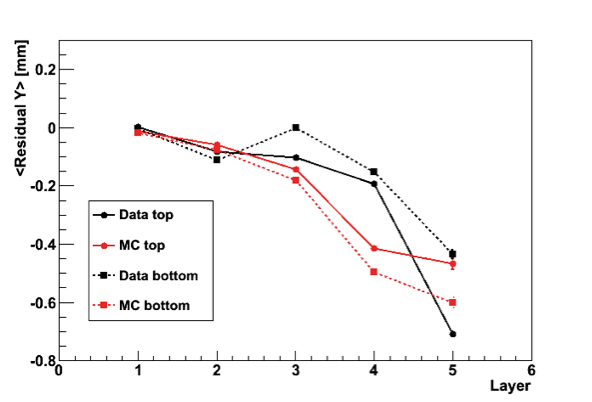
\includegraphics[ scale=0.7]{test2012/alignment/pictures/res_top/res_top_summary-1.png}
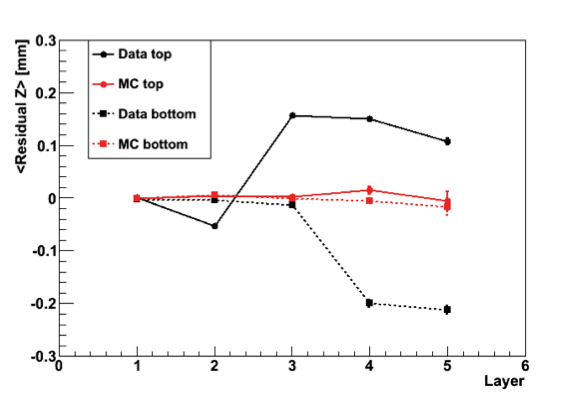
\includegraphics[ scale=0.7]{test2012/alignment/pictures/res_top/res_top_summary-2.png}\caption{\small{Mean of the track residuals for each detector layer in the top tracker half 
in the bend (left) and non-bend (right) plane.}}\label{fig:res_top_summary}
\end{figure*}
 Note also that larger width for the later layers which highlights the large 
multiple scattering contribution in the previous layers. The estimation of the 
uncertainty due to multiple scattering can also be seen in the track residual 
pull which is defined as the track residual divided by the estimated hit position 
uncertainty. These are shown in Fig.~\ref{fig:res_pull_top_nonbend} and~\ref{fig:res_pull_top_bend}.
The intrinsic single hit resolution of $\approx 6~\mu$m is negligible 
for layers beyond the second. Note that these pull distributions come from biased 
residuals (the hit was used in the track fit) and are thus not expected to have a 
width of one. 
\begin{figure*}[t]
%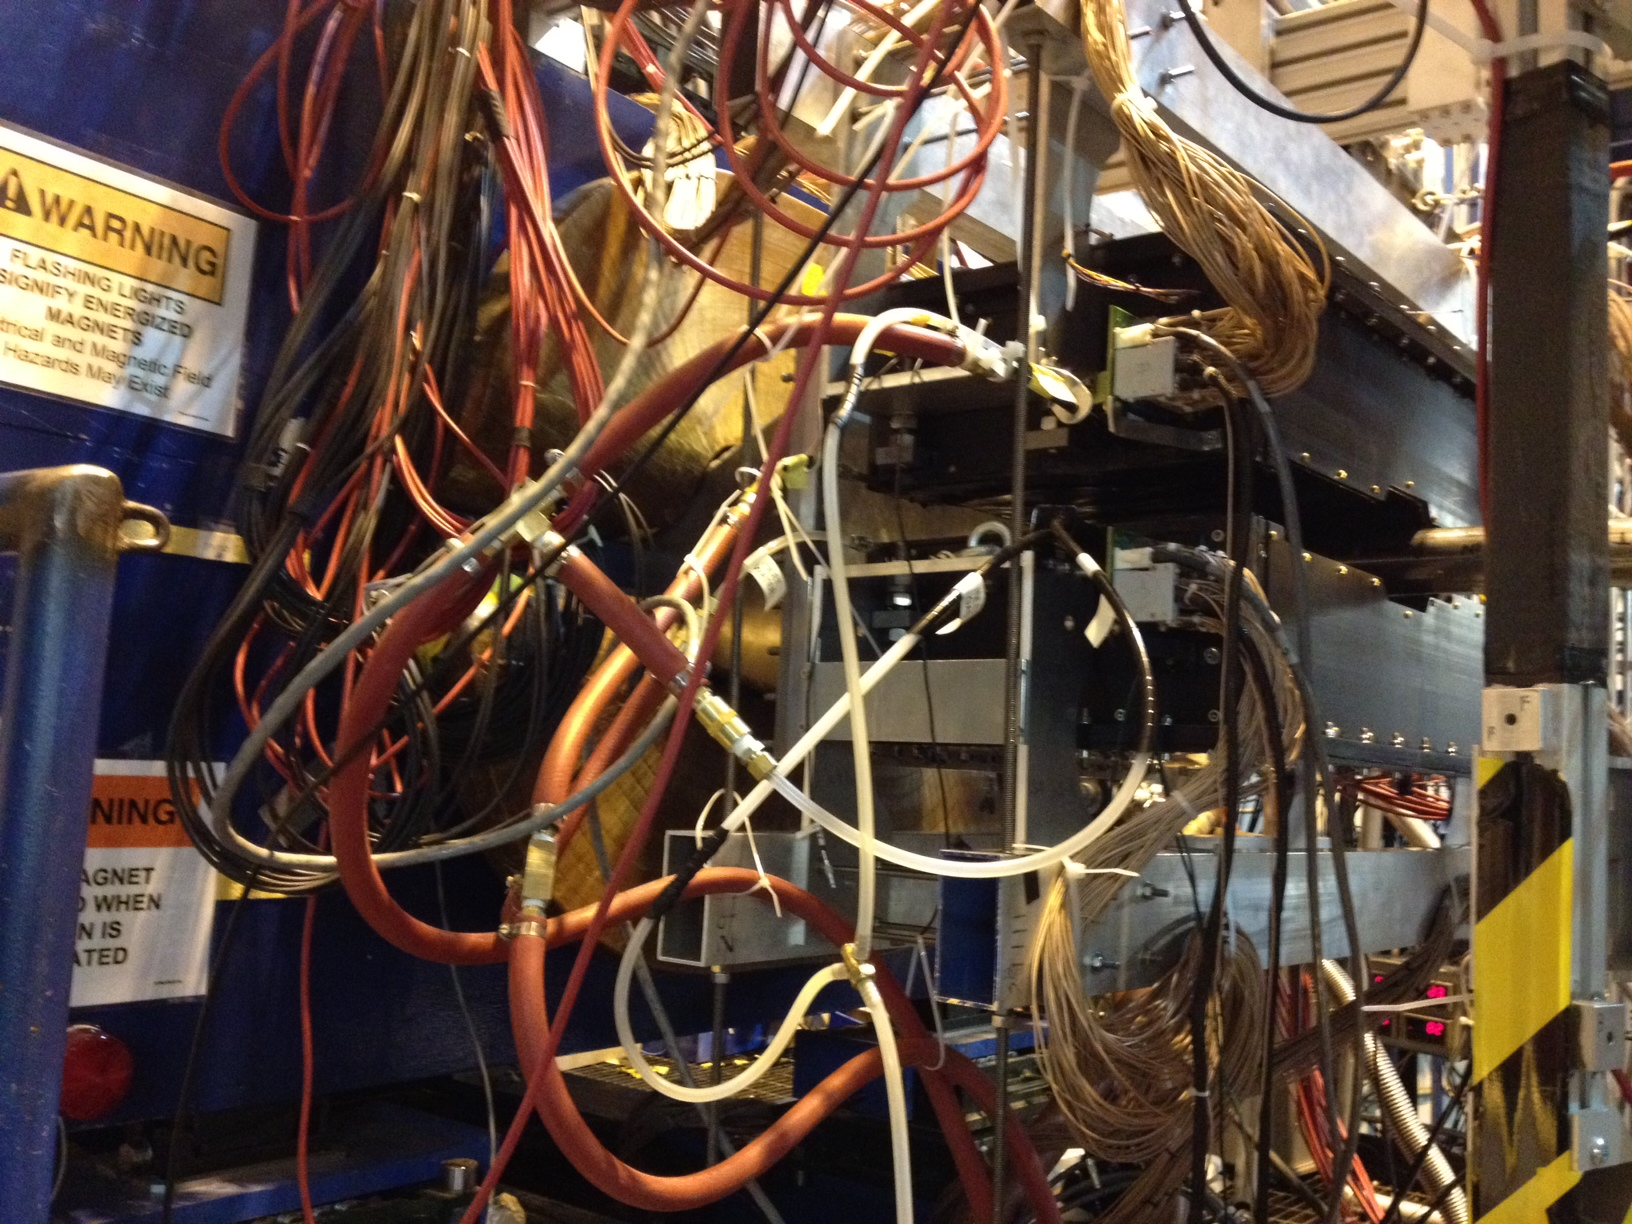
\includegraphics[ scale=0.25]{test2012/ecal_mounted.JPG}
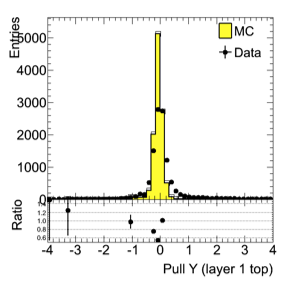
\includegraphics[ scale=0.5]{test2012/alignment/pictures/res_pull_top/res_pull_top-1.png}
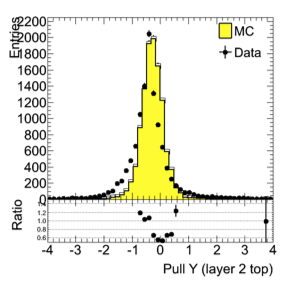
\includegraphics[ scale=0.5]{test2012/alignment/pictures/res_pull_top/res_pull_top-2.png}
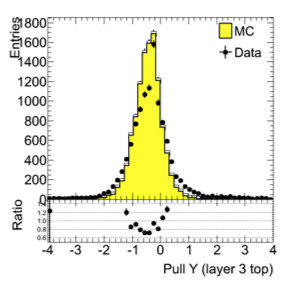
\includegraphics[ scale=0.5]{test2012/alignment/pictures/res_pull_top/res_pull_top-3.png}
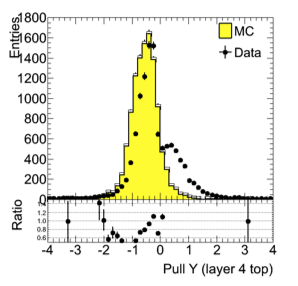
\includegraphics[ scale=0.5]{test2012/alignment/pictures/res_pull_top/res_pull_top-4.png}
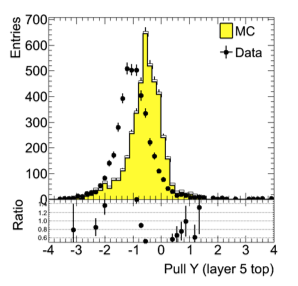
\includegraphics[ scale=0.5]{test2012/alignment/pictures/res_pull_top/res_pull_top-5.png}
\caption{\small{Residuals in the bend plane for tracks reconstructed in the 
top half of the tracker. }}\label{fig:res_pull_top_bend}
\end{figure*}
\begin{figure*}[t]
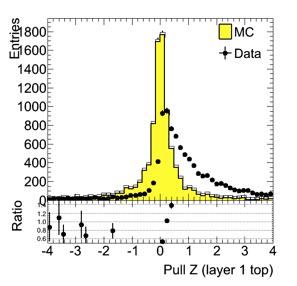
\includegraphics[ scale=0.5]{test2012/alignment/pictures/res_pull_top/res_pull_top-6.png}
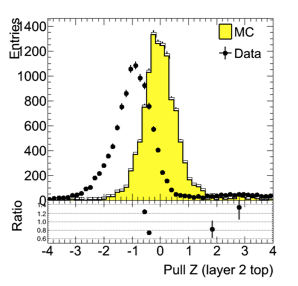
\includegraphics[ scale=0.5]{test2012/alignment/pictures/res_pull_top/res_pull_top-7.png}
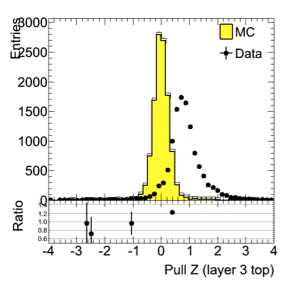
\includegraphics[ scale=0.5]{test2012/alignment/pictures/res_pull_top/res_pull_top-8.png}
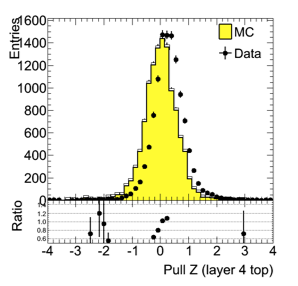
\includegraphics[ scale=0.5]{test2012/alignment/pictures/res_pull_top/res_pull_top-9.png}
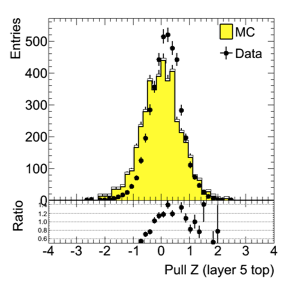
\includegraphics[ scale=0.5]{test2012/alignment/pictures/res_pull_top/res_pull_top-10.png}
\caption{\small{Residuals in the non-bend plane for tracks reconstructed in the 
top half of the tracker.  }}\label{fig:res_pull_top_nonbend}
\end{figure*}

The residuals give information on the internal alignment of the tracker. It is important 
to understand the tracker alignment w.r.t. to the other components in the beam line. 
This can be achieved by using the fitted tracks and extrapolate them outside the tracking 
volume. Figure~\ref{fig:test_harpscan} shows a HARP scan taken during the test run. 
\begin{figure*}[t]
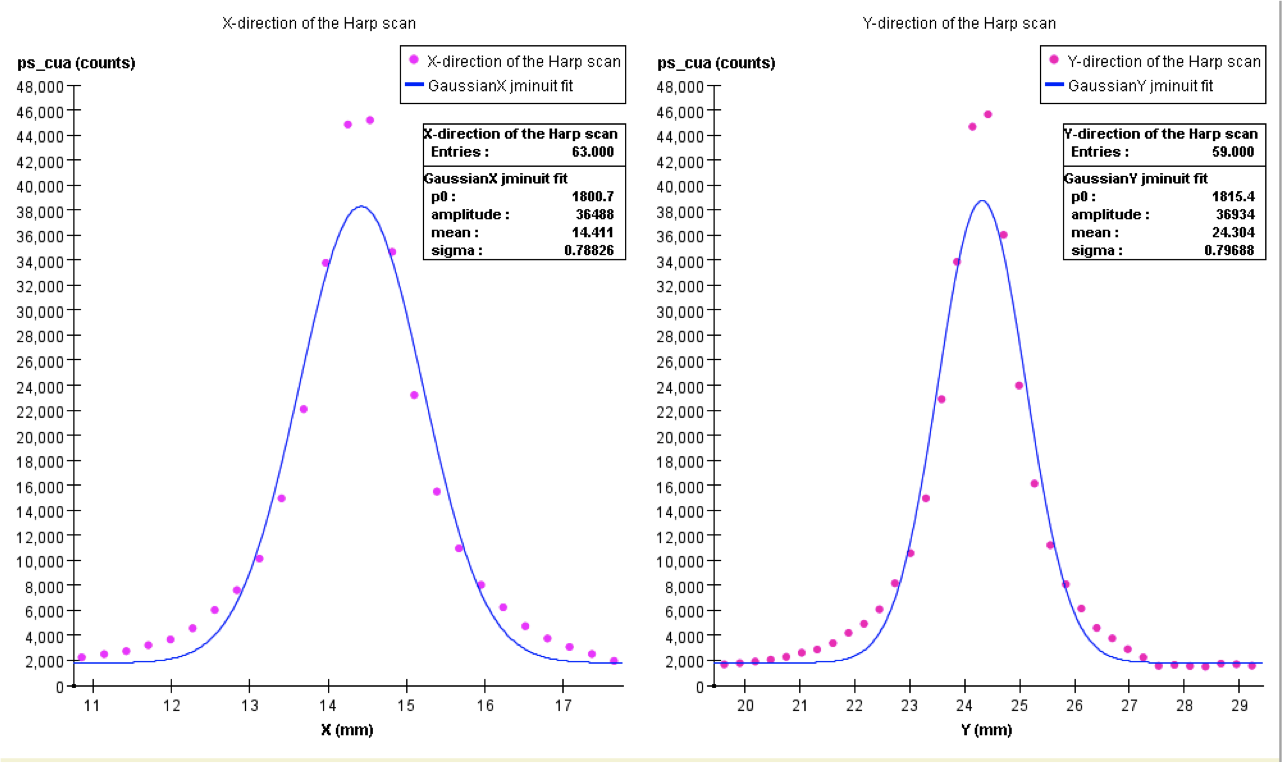
\includegraphics[ scale=0.5]{test2012/alignment/pictures/harp_scan_testrun.png}
\caption{\small{Photon beam profile HARP scan close to the converter.}}\label{fig:testrun_harpscan}
\end{figure*}
The width of the beam can be described by a double Gaussian $0.71e^{\frac{x}{0.366}}\times 0.29e^{1.111}$ which is also used in the simulations. The beam envelope extends out to 
about 7mm. By extrapolating the fitted tracks to the converter position along the beam 
we get a feeling for our alignment of the tracker w.r.t. to the beam line. This is shown in 
Fig.~\ref{fig:extrapol_converter_X}.
\begin{figure*}[t]
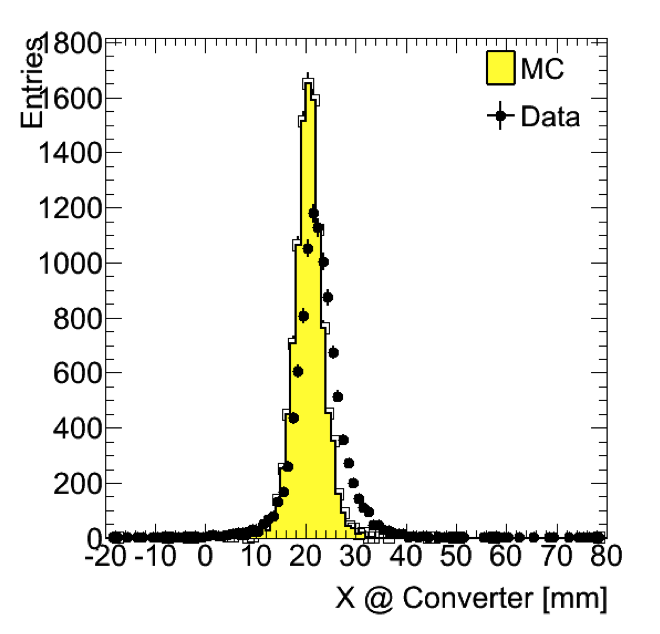
\includegraphics[ scale=0.5]{test2012/alignment/pictures/extrapolation_converter/extrapolation_X_converter_top.png}
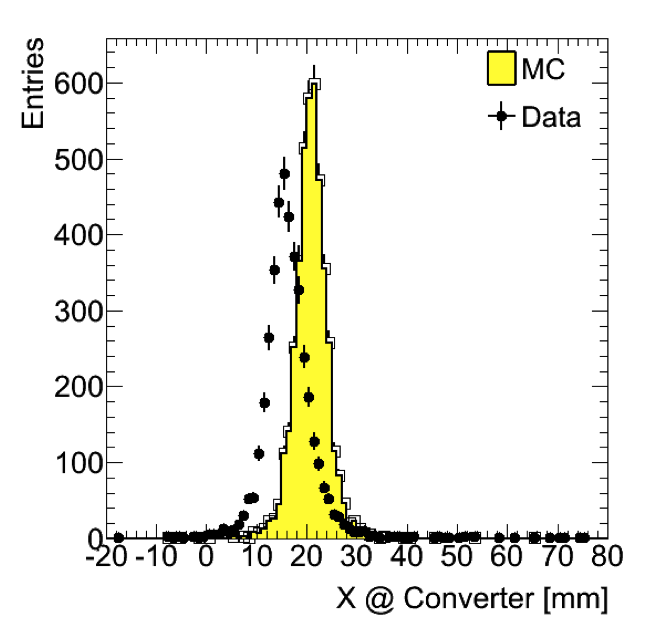
\includegraphics[ scale=0.5]{test2012/alignment/pictures/extrapolation_converter/extrapolation_X_converter_bot.png}
\caption{\small{Extrapolated track position in the bend plane direction.}}
\label{fig:extrapol_converter_X:}
\end{figure*}
\begin{figure*}[t]
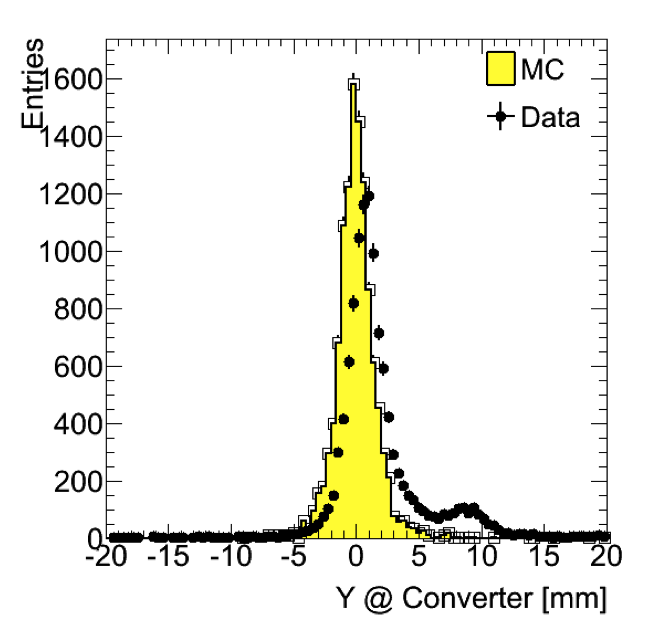
\includegraphics[ scale=0.5]{test2012/alignment/pictures/extrapolation_converter/extrapolation_Y_converter_top.png}
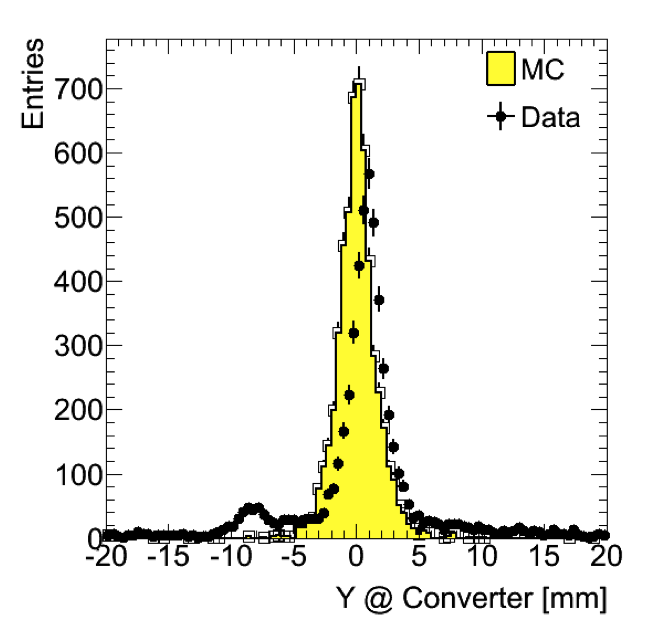
\includegraphics[ scale=0.5]{test2012/alignment/pictures/extrapolation_converter/extrapolation_Y_converter_bot.png}
\caption{\small{Extrapolated track position in the non-bend plane direction.}}
\label{fig:extrapol_converter_Y}
\end{figure*}
